%% =====================================================================
%%  Physical Review Research (PRR) submission
%%  APS REVTeX 4.2 document class, apsrev4-2 bibliography style.
%%
%%  This file re-formats paper/main.tex into the APS/PRR layout.
%%  It reuses every existing section file unchanged (including the
%%  abstract file); only the class, front matter, and reference style
%%  differ from the original.
%%
%%  Layout notes:
%%    * [reprint]  = two-column journal look (used here).
%%      Switch to [preprint] for a single-column, double-spaced draft.
%%    * All figures are six-panel composites, so the {figure}
%%      environment is globally promoted to {figure*} (full page
%%      width) without touching the section sources.
%% =====================================================================
%% showkeys is required for \keywords to be typeset; without it REVTeX
%% silently drops them (and warns in the log).
\documentclass[aps,prresearch,reprint,superscriptaddress,longbibliography,%
               nofootinbib,showkeys]{revtex4-2}

%% --- Mathematics and graphics ---
\usepackage{amsmath}
\usepackage{amssymb}
\usepackage{mathtools}
\usepackage{bm}
\usepackage{graphicx}
\usepackage{booktabs}
\usepackage{microtype}

%% --- Cross-document references into the Supplemental Material ---
\usepackage{xr-hyper}
\usepackage[hidelinks]{hyperref}
\externaldocument{supplement_prr}[supplement_prr.pdf]

%% Float placement: STYLE_GUIDE 1.3 recommends relaxing the float
%% parameters, but that remedy targets documents whose figures pile up after
%% the conclusion.  Here the defaults already interleave all six figures
%% (pages 3,4,5,7,8,9 with the conclusion on page 14); forcing the relaxed
%% parameters spread the same content over two extra pages, so they are not
%% applied.

%% --- Project macros, computed values, and the shared caption registry ---
% Shared semantic notation. Computed values are exported separately to
% paper/generated/results_macros.tex.
% Suppress engine-generated timestamps, trailer IDs, and PTEX provenance so
% SOURCE_DATE_EPOCH-controlled builds are byte reproducible.
\ifdefined\pdfinfoomitdate
  \pdfinfoomitdate=1
\fi
\ifdefined\pdftrailerid
  \pdftrailerid{}
\fi
\ifdefined\pdfsuppressptexinfo
  \pdfsuppressptexinfo=-1
\fi
\newcommand{\ZGV}{ZGV}
\newcommand{\MorseBott}{Morse--Bott}
\newcommand{\kvec}{\bm{k}}
\newcommand{\xvec}{\bm{x}}
\newcommand{\uvec}{\bm{u}}
\newcommand{\nvec}{\bm{n}}
\newcommand{\dd}{\mathop{}\!\mathrm{d}}
\newcommand{\ii}{\mathrm{i}}
\newcommand{\ee}{\mathrm{e}}
\newcommand{\order}{\mathcal{O}}
\newcommand{\abs}[1]{\left\lvert #1 \right\rvert}
\newcommand{\norm}[1]{\left\lVert #1 \right\rVert}
\DeclareMathOperator{\Hess}{Hess}
\DeclareMathOperator{\diag}{diag}
\DeclareMathOperator{\sgn}{sgn}

\newcommand{\ZGVKappa}{0.804217}
\newcommand{\ZGVOmega}{2.85176}
\newcommand{\ZGVCurvature}{1.19686}
\newcommand{\VFour}{0.0140638}
\newcommand{\SplittingSlope}{0.995817}
\newcommand{\RemainderSlope}{1.99957}
\newcommand{\EarlyDecaySlope}{-0.518693}
\newcommand{\LateDecaySlope}{-0.965731}
\newcommand{\MaxPhaseError}{1.28586\times10^{-6}}
\newcommand{\MorseMinimumCount}{4}
\newcommand{\MorseSaddleCount}{4}

% Central caption registry shared by the main paper and Supplementary Information.

\newcommand{\FigureOneCaption}{Mechanism overview on the selected branch.
\textbf{a}, Thin grey contours show the isotropic full-wave local-frequency
surface, and the solid grey curve marks the continuous ZGV ring at the exact
isotropic radius \(\kappa_0\).  \textbf{b}, Angular anomaly of the perturbation: the difference between
the anisotropic and isotropic surfaces with its mean over angle removed at
each radius.  The removed part is the angle-independent carrier shift,
which moves the ring without breaking it, so the fourfold remainder shown
here is the part that breaks it.  Troughs and crests are shaded in the
minimum and saddle colours; the computed, independently refined minima
(blue circles) and saddles (orange diamonds) fall on the troughs and
crests respectively, within the declared local annulus.  Marker shape
duplicates colour, and the panel regroups the two stored surfaces without
introducing a new computation.  \textbf{c}, Conceptual summary of the
change from a one-dimensional critical ring with generic \(t^{-1/2}\) decay to
isolated Morse points with generic \(t^{-1}\) decay; this panel is explanatory
rather than numerical, with the computed asymptotic slices tested in
Fig.~\ref{fig:decay-crossover}.  This mechanism overview does not carry the
numerical realization claim; the finite-resolution full-wave search,
Cartesian Hessians, and stability checks are reported in
Fig.~\ref{fig:morse-points}.  Wavevector components are normalized as
\(k_xh\) and \(k_yh\), frequencies as \(\Omega=\omega h/c_T\), and panels
\textbf{a} and \textbf{b} use common axes.  Source data:
\texttt{data/source\_data/figure\_01}.}

\newcommand{\FigureTwoCaption}{Independent numerical verification of the
isotropic reference.  \textbf{a}, The solid curve is the independently
discretized full-wave symmetric branch; the open orange circular symbol marks
the exact Rayleigh--Lamb reference \((\kappa_0,\Omega_0)\).  \textbf{b}, The
solid curve with circular markers is the local full-wave branch, whereas the
dashed line is the coefficient prediction
\(\Omega_0+a(\kappa-\kappa_0)^2/2\).  The positive curvature \(a\) is obtained
from exact implicit differentiation, not from a fit to the plotted samples.
\textbf{c}, Coloured marker--lines on the left axis report relative
\(\kappa_0\), \(\Omega_0\), and curvature errors together with the normalized
eigen residual, Hermitian defect, and mass-orthogonality defect; the
short-dashed line on the right axis is the relative eigengap.  \textbf{d},
Through-thickness profiles of the mass-normalized mode: solid, short-dashed,
and long-dashed curves denote \(\lvert u_x\rvert\), \(\lvert u_y\rvert\), and
\(\lvert u_z\rvert\), divided by their common global maximum.  The neutral
dotted curve is the squared-displacement proxy \(\sum_i\lvert u_i\rvert^2\),
normalized by its own maximum; it is neither a signed-parity nor a strain-energy
diagnostic.  Here \(\kappa=kh\), \(\Omega=\omega h/c_T\), and \(z/h\) is the
normalized thickness coordinate.  Source data:
\texttt{data/source\_data/figure\_02}.}

\newcommand{\FigureThreeCaption}{Full-elastic sensitivities for the declared
weak cubic family.  \textbf{a}, The solid curve is the analytic full-elastic
coefficient \(V(\theta)-V_0\), and the dashed curve is
\(V_4\cos(4\theta)\).  A common radial offset is used only to render the polar
plot, and the rings are drawn unlabelled; the outermost petal reaches
\(\lvert V_4\rvert\) in units of \(\Omega/\varepsilon\), whose value is
given in panel \textbf{c}.  \textbf{b}, Stems and circular markers show every
stored harmonic amplitude \(\lvert V_m\rvert\) on a logarithmic scale; the
\(m=4\) marker is highlighted and non-fourfold leakage is retained.
\textbf{c}, Filled circles show the stored physical shift
\(\varepsilon V_4\), while the dashed line shows \(Q_4\Delta_C\).  Their
agreement checks the perturbation convention
\(V_4=Q_4\Delta_C^{(1)}\) and
\(\Delta_C=\varepsilon\Delta_C^{(1)}\), rather than providing an independent
full-wave comparison.  \textbf{d}, Solid lines are the analytic full-elastic
\(V\) and \(B=\partial_\kappa V\); open circles and squares are independent
centered full-wave finite differences.  Agreement is quantified by the relative errors
\(\lVert V_{\rm FD}-V\rVert_2/\lVert V\rVert_2\) and
\(\lVert B_{\rm FD}-B\rVert_2/\lVert B\rVert_2\), which the build asserts
to lie below the registered tolerance.  The inset gives the
declared centered-difference step convergence of the relative \(V_4\) and
\(B\) errors.  Source data: \texttt{data/source\_data/figure\_03}.}

\newcommand{\FigureFourCaption}{Full-wave numerical realization of the local
Morse splitting with eight resolved roots.  \textbf{a}, Grey contours show the isotropic full-wave surface,
the solid grey curve marks the exact isotropic critical ring, and the two
short-dashed circles delimit the declared annulus.  \textbf{b}, Filled and
line contours show the anisotropic full-wave surface using the same levels as
panel \textbf{a}; blue circles and orange diamonds are the stored refined
minima and saddles, and the short-dashed circles again show the annular
boundaries.  \textbf{c}, Cartesian Hessian eigenvalues are ordered by
critical-point angle on a symmetric logarithmic axis.  Marker shape and colour
identify Morse class, filled and open symbols denote \(\lambda_1\) and
\(\lambda_2\), vertical bars give the declared Hessian-discrepancy estimate,
and the shaded band spans the maximum such estimate about zero.
\textbf{d}, Filled symbols joined by the solid guide line give the signed
radial error
\((\kappa_{\rm full}-\kappa_{\rm pert})/\kappa_0\); open symbols joined by the
dashed guide line give the signed frequency error
\((\Omega_{\rm full}-\Omega_{\rm pert})/\Omega_0\).  The perturbation values
are first-order predictions, and neither guide line is a fit.  All surfaces
and coordinates use the normalized \(kh\) and \(\omega h/c_T\) convention.
Source data: \texttt{data/source\_data/figure\_04}.}

\newcommand{\FigureFiveCaption}{Perturbation checks over the complete
declared weak-anisotropy sequence.  \textbf{a}, Open circles are the
full-wave minimum--saddle frequency splitting, and the dashed line is its
first-order coefficient prediction.  The reported splitting slope is an
unweighted log--log fit over every declared positive \(\lvert\varepsilon\rvert\),
not a plot-selected range; no separate fitted line is drawn.  \textbf{b}, Blue
circles and orange diamonds show the baseline-corrected full-wave radial shifts
\(q_{\min}/\varepsilon\) and \(q_{\rm sad}/\varepsilon\), while the
corresponding dashed lines are the coefficient limits
\(-B(\theta_j)/a\).  The annotated radial slope is obtained from the
uncompensated quantity \(\max(\lvert q_{\min}\rvert,\lvert q_{\rm sad}\rvert)\)
over the same complete sequence.  \textbf{c}, Markers and connecting guide
lines show the absolute full-wave minus first-order critical-frequency errors
divided by \(\varepsilon^2\) for the minimum and saddle families.  The
reported remainder slope is fitted to the maximum uncompensated error across
the two families; the connecting lines are not fits.  \textbf{d}, Circle and
diamond markers show the minimum and saddle angular orbits for opposite
perturbation signs, demonstrating exchange of the axis and diagonal roles
under \(\varepsilon\rightarrow-\varepsilon\).  Source data:
\texttt{data/source\_data/figure\_05}.}

\newcommand{\FigureSixCaption}{Two numerical asymptotic slices of the
coefficient-resolved response \(G^+\), with \(t=t_{\rm phys}c_T/h\).
\textbf{a}, Full-wave real parts and magnitudes, after removal of the shifted
carrier \(\Omega_0+\varepsilon V_0\) and uniform scaling, collapse onto
\(J_0(\tau)\), \(\tau=\varepsilon V_4t\), for the four declared uniform
transition rows.  The comparison is performed without fitted alignment.
\textbf{b}, Thin curves show the absolute complex error at all stored times;
thick segments show the uniform transition window \(t\geq1500\),
\(\lvert\tau\rvert\leq2\), including Bessel zeros.  \textbf{c}, Pale bands mark the two fitted
intervals.  The early fit
uses the raw \(\varepsilon=0.005\) magnitude, whereas the late fit uses four
complete beat-period RMS values in the fixed-anisotropy
\(\varepsilon=0.08\) row.
These are two slices, not one numerical time trajectory; the proved
growing-\(\lvert\tau\rvert\) overlap connects their coefficients and phases.
\textbf{d}, Crossover markers are first downward crossings of magnitude
\(0.9\) within a theory-centred bracket.  This is a theory-centred consistency
diagnostic; panel \textbf{a} is the primary numerical test.  \textbf{e}, At
\(\varepsilon=0.08\), the full integral and exact-Hessian Morse sum are compared
over \(1500\leq t\leq10200\); open markers denote cancellation samples with
coherence below \(0.30\).  \textbf{f}, Exact minimum and saddle frequencies
mark the critical-frequency features.  Their separation is
\(2\lvert\varepsilon V_4\rvert\) and the modulation magnitude is
\(\lvert\varepsilon V_4\rvert\).  Source data:
\texttt{data/source\_data/figure\_06}.}

\newcommand{\SupplementaryFigureOneCaption}{Polynomial-order and assembly
cross-checks for the selected isotropic branch.  \textbf{a}, Solid
marker--lines give relative errors in the exact Rayleigh--Lamb reference
\(\kappa_0\) (blue circles), \(\Omega_0\) (orange squares), and curvature
\(a\) (dark-blue diamonds) on logarithmic axes.  Each reported fine GLL order
\(p\) pairs a tracked evaluator at \(p-4\) with its independent diagnostic at
\(p\); the machine-precision plateaux need not be monotone.  \textbf{b}, The
same colours and markers show an independently reconstructed one-element
spectrum, while the coloured stars at the final order report the independent
two-element result.  \textbf{c}, At the shared final order, grey circles and
dark-blue stars compare the one- and two-element errors for all three
quantities.  The declared gates are relative \(\kappa_0\) and \(\Omega_0\)
errors below \(10^{-7}\), relative curvature error below \(10^{-4}\), eigen
residual below \(10^{-10}\), and relative eigengap greater than ten times the
larger of that residual and machine precision.  These are local discretization
and mesh-split diagnostics, not a proof for the complete spectrum.  Source
data: \texttt{data/source\_data/supplementary}.}

\newcommand{\SupplementaryFigureTwoCaption}{Quadrature, interpolation, and
phase-discrepancy convergence for the declared response window.  All panels use
the nested angular--radial grids \((N_\theta,N_q)=(16,65),(32,129),(64,257)\)
and a \((128,513)\) reference surface; solid curves with circular markers and
logarithmic ordinates show directly computed diagnostics.  \textbf{a}, Blue
circles give the RMS norm of the coarse-minus-reference demodulated complex
full-wave response divided by the reference-response RMS over the declared
time samples.  \textbf{b}, Blue circles give the maximum absolute frequency
error after periodic-angular and cubic-radial interpolation of each coarse
surface onto the reference grid.  \textbf{c}, Orange circles give the
accumulated inter-resolution phase-discrepancy estimator at the declared
maximum time, including interpolation and coarse/reference nested-order
frequency differences; the black short-dashed line is the declared acceptance
threshold of \(0.05\) rad.  The finest
quadrature error is required to be at most \(0.05\), and successive quadrature
and interpolation ratios at most one half.  These empirical estimators test
consistency across computed resolutions; they do not bound the unknown
continuum error or imply infinite-time phase accuracy.  Source data:
\texttt{data/source\_data/supplementary}.}

\newcommand{\SupplementaryFigureThreeCaption}{Local branch-tracking and
simple-eigenvalue diagnostics.  \textbf{a}, The solid blue curve with circles
is the mass-weighted modal assurance criterion relative to the \(\kappa_0\)
anchor over the declared local wavenumber window; the acceptance threshold
is \(0.99\).  \textbf{b}, The solid orange curve with diamonds is the relative
eigengap of the same tracked branch over that window.  \textbf{c}, On a
logarithmic ordinate, black circles and a solid line report the eigengap and
dark-blue squares and a solid line report the normalized eigen residual over
the polynomial-order sweep.  Acceptance requires residual below \(10^{-10}\)
and gap greater than ten times the larger of residual and machine precision.
Together these computed quantities support branch continuity and separation
only near the selected ZGV point; they neither identify the branch globally
nor certify unrelated modes.  Source data:
\texttt{data/source\_data/supplementary}.}

\newcommand{\SupplementaryFigureFourCaption}{Independent finite-difference
closure of the analytic generalized-eigenvalue sensitivities.  The horizontal
step axes in panels \textbf{a} and \textbf{b} are reversed so refinement runs
from left to right.  \textbf{a}, Blue circles and a solid line show the
centered-difference relative error in \(V_4\) versus
\(\Delta\varepsilon\).  \textbf{b}, Orange circles and a solid line show the
paired-step diagonal error in \(B\), defined as the Euclidean relative error
of the two-component vector at \(\theta=0\) and \(\pi/4\) when
\(\Delta\varepsilon=\Delta q\).  \textbf{c}, The logarithmically coloured
tensor-product heatmap reports the same vector error for every pair
\((\Delta\varepsilon,\Delta q)\); darker cells denote larger error and printed
annotations give the numerical values.  The sensitivity tolerance is \(10^{-4}\):
the final two \(V_4\) steps and the finest two-by-two \(B\) block satisfy it.
These full-wave centered differences are independent of the analytic
sensitivity formula, although they use the same full-wave eigensolver; they
are not fitted data.  Source data:
\texttt{data/source\_data/supplementary}.}

\newcommand{\SupplementaryFigureFiveCaption}{Sensitivity of the computed
response norm to the declared source and spectral window class.  Each ratio
uses the RMS of the demodulated complex full-wave response over the declared
time samples at \(\varepsilon=0.02\), normalized by the baseline
\((R/h,\sigma/k_0)=(0.5,0.15)\).  \textbf{a}, The annotated heatmap covers
three source radii and three super-Gaussian widths; the diverging colour scale
is centered on the normalized baseline value one.  \textbf{b}, Solid curves
with circular markers show the same ratios against \(R/h\), with colour
distinguishing \(\sigma/k_0\); the black horizontal line is the declared
baseline.  The separately computed widest-window boundary weight is required
to remain below the truncation gate \(5\times10^{-3}\).  This sweep supports
response-norm robustness within the displayed source--window class only.  It
does not establish source independence and is not evidence for either the
crossover exponents or the Morse theorem.  Source data:
\texttt{data/source\_data/supplementary}.}

\newcommand{\SupplementaryFigureSixCaption}{Finite-anisotropy silicon stress
test outside the weak-anisotropy theorem, for a [001] plate with
\(C_{11}=165.7\), \(C_{12}=63.9\), and \(C_{44}=79.6\,\mathrm{GPa}\)
(material source \texttt{doi:10.1107/S1600577514004962}).  \textbf{a}, Filled
blue shading and blue contour lines show the full-wave local-frequency surface
normalized as \(\Omega=\omega h/\sqrt{C_{44}/\rho}\); blue circles and orange
diamonds mark four refined minima and four saddles within the declared
annulus.  The shading is not a
separate quantitative colour scale.  \textbf{b}, Points are ordered by stored
index; orange circles and a solid line show the Cartesian Hessian eigenvalue
\(\lambda_1\), blue squares and a solid line show \(\lambda_2\), and the black
line marks zero.  Here marker identity denotes eigenvalue rather than Morse
class: both values are positive at minima and have opposite signs at saddles.
\textbf{c}, On a logarithmic axis, blue circles and a solid line give the
relative tracking gap, while orange diamonds and a solid line give the
stationarity residual \(\lVert\nabla_{\boldsymbol{k}}\Omega\rVert\); this panel
does not display the separately evaluated annular-boundary consistency check.
This is a finite-anisotropy stress test of the numerical search and local
classification only, not evidence for the weak-anisotropy theorem.  Source
data: \texttt{data/source\_data/supplementary}.}

%% Figures are authored at 183 mm; the REVTeX text block is 510 pt
%% (180 mm), so placing them at full \textwidth renders them at their
%% design size.  The former 0.90 factor shrank every figure by a
%% further 10% and with it all in-figure type (STYLE_GUIDE 3.8).
\newcommand{\SixPanelFigureWidth}{\textwidth}

%% --- Promote every figure to span both columns (six-panel figures) ---
\makeatletter
\renewenvironment{figure}[1][tbp]{\begin{figure*}[#1]}{\end{figure*}}
\makeatother

\begin{document}

\title{A Coefficient- and Phase-Resolved Bridge across Noncommuting
Limits of Lamb-Wave ZGV Splitting}

%% ===== Authors and affiliations: FILL IN before submission =========
\author{Author One}
\email{author.one@example.edu}
\affiliation{Department of Mechanical Engineering, Example University,
City 00000, Country}

\author{Author Two}
\affiliation{Department of Mechanical Engineering, Example University,
City 00000, Country}
%% ===================================================================

%% REVTeX takes the "Dated: " prefix as \date's optional argument, so
%% clearing both prefix and body suppresses the line entirely; \date{}
%% alone still typesets an empty "(Dated:)".
\date[]{}

%% Keywords: PRR prints these under the abstract.  Terms chosen to match
%% the vocabulary of the paper itself rather than generic field labels.
%% REVTeX separates keywords with commas; \sep is Elsevier syntax.
\keywords{Lamb waves, zero-group-velocity resonance, cubic anisotropy,
Morse--Bott unfolding, guided-wave asymptotics}

%% REVTeX requires the abstract before \maketitle; the original
%% abstract file already provides the {abstract} environment verbatim.
\begin{abstract}
Breaking continuous rotational symmetry changes the dimension of a stationary
set and can make the symmetry-restoring and long-time limits noncommuting.  In
isotropic Lamb waves, a finite-wavenumber zero-group-velocity (ZGV) critical
ring produces a radial \(t^{-1/2}\) response, whereas cubic anisotropy resolves
the ring into isolated Morse points with an ultimate \(t^{-1}\) response.
These endpoints were known.  Our dated literature audit found no prior plate
calculation joining their full-elastic coefficients, normalization, and
signature phases under the controls used here.  We derive that bridge for a
selected simple, uniformly gapped branch.
Generalized-eigenvalue sensitivities determine the angular and radial coefficients, and a
Morse--Bott reduction proves \(\MorseMinimumCount\) minima and
\(\MorseSaddleCount\) saddles for sufficiently small nonzero perturbations.  A
finite-resolution calculation yields eight resolved, refinement-stable roots
without asserting continuum exhaustion.  After removal of the shifted carrier
\(\Omega_0+\varepsilon V_0\), direct branch quadrature follows
\(t^{-1/2}J_0(\varepsilon V_4t)\); a separately evaluated fixed-anisotropy slice
approaches the exact-Hessian Morse sum, and a proved growing-parameter overlap
matches their coefficients and phases.  The comparisons are performed without
fitted alignment.  Their largest accumulated inter-resolution
phase-discrepancy estimator is \(\MaxPhaseError\,\mathrm{rad}\); this empirical
quantity is not a continuum error bound.  The computation-only result is
restricted to a linear, lossless infinite plate, the declared local annulus,
and the specified source and weak-anisotropy classes.
\end{abstract}


\maketitle

\section{Introduction}

Finite-wavenumber zero-group-velocity (ZGV) Lamb states are central to
long-lived localization in plates.  They retain a nonzero in-plane wavelength
while a stationary guided-wave dispersion suppresses the
leading transport of energy away from the source, producing local vibration
and a temporal decay law controlled by the geometry of the stationary set.
Laser-ultrasonic excitation and local ZGV responses are established
phenomena \citep{prada2005laser,prada2008local}.  In an isotropic plate,
rotational symmetry turns a radial finite-wavenumber stationary point into a
continuous ZGV critical ring, and radial stationary phase gives the established
\(t^{-1/2}\) decay for a nonnodal local response
\citep{prada2008power,laurent2014temporal}.  Neither the ZGV critical ring nor
this exponent is at issue here as a new effect; they provide the known
isotropic endpoint whose loss of directional degeneracy we examine.

Elastic anisotropy provides the other established endpoint.  Anisotropic-plate
studies established directional ZGV shifts \citep{prada2009anisotropy}.
Calculations also found multiple stationary points
\citep{hussain2012multiple,karous2019multiple}, and isolated anisotropic ZGV
points were previously reported.  More specifically, four minima and four saddles, together with
their interference, were previously reported for a cubic silicon plate
\citep{kiefer2023beating}; subsequent work described their directional
stationary-phase organization and unfolding \citep{kiefer2025skewing}.
Algorithms for computing isolated ZGV points in the full guided-wave spectrum
are likewise established \citep{kiefer2023computing,plestenjak2025sylvester}.
The present calculation therefore does not claim the isolated points, their
alternating four-plus-four organization, or the associated interference as
new observations.  Its question is how these known anisotropic objects emerge
in a controlled limit from the known isotropic ZGV critical ring.

A plate-specific question remains open in the literature examined here: how to
construct a coefficient-resolved connection between that geometry and the
temporal asymptotics of the full Lamb eigenproblem.
Morse--Bott critical manifolds and their perturbations are established
mathematics \citep{bott1954critical,banyaga2013cascades}, while
two-dimensional stationary phase has long been applied to isolated guided-wave
points \citep{velichko2007excitation,chapuis2010focusing,
karmazin2013caustics}.  Broken-symmetry uniform approximations in other wave
settings also connect continuous families to isolated objects through a
Bessel modulation \citep{creagh1996broken,brack1999uniform,brack2009closed}.
The required connection must retain full-elastic angular and radial
coefficients, a derivative-level remainder, source normalization, and a
phase-controlled temporal comparison.  This missing link, rather than a new
general Morse or Bessel theorem, is the focus of the analysis.

Here we connect the known ZGV critical ring to the anisotropic endpoint.  The
reduction treats weak cubic anisotropy on a simple tracked Lamb branch.
Full-elastic generalized-eigenvalue sensitivities determine the angular
coefficient \(V_4\) and the radial coefficient \(B\) without fitting.
Critical-point geometry, Cartesian Hessian inertia, and annular index
checks then test the alternating local Morse set and its perturbative
scaling inside a declared local annulus.  Uniform Bessel asymptotics connect
the ring response to the isolated-point regime, while the fixed-anisotropy
endpoint retains exact critical frequencies and Hessians.  Finally, validated
spectral computations and an accumulated inter-resolution phase-discrepancy
estimator test the entire chain without fitted amplitude, phase, frequency, or
time shifts.  The study is
computation-only: it concerns one selected simple branch and a controlled
weak-anisotropy family; the finite-anisotropy silicon stress test is separate
from the asymptotic evidence.

\section{The Isotropic ZGV Ring}

\subsection{Exact Rayleigh--Lamb reference}

We restrict the isotropic reference calculation to the selected symmetric
$S_1$ branch and the configured local window around its zero-group-velocity
(ZGV) state.  Within that scope, the traction-free Rayleigh--Lamb determinant
is desingularized before root finding, so a vanishing shear thickness
wavenumber cannot be mistaken for a physical root.  With
$\kappa=kh$ and $\Omega=\omega h/c_T$, simultaneously solving
$D_S=D_{S,k}=0$ gives the dimensionless location
$\kappa_0=\ZGVKappa$ and frequency $\Omega_0=\ZGVOmega$; implicit
differentiation gives the positive dimensionless radial curvature
$a=\mathrm d^2\Omega/\mathrm d\kappa^2=\ZGVCurvature$.  These quantities
characterize one simple local branch,
not all symmetric, antisymmetric, or shear-horizontal branches of the plate.

The reference starts from the physical face-traction matrix rather than a
quotient form of the classical dispersion relation
\citep{lamb1917waves}.  Rescaling the shear potential produces the regular
determinant in Eq.~\eqref{eq:desingularized-determinant}, which remains finite
through the shear cutoff.  The nonzero frequency derivative then identifies a
smooth scalar branch, while Eqs.~\eqref{eq:implicit-first-derivative} and
\eqref{eq:zgv-curvature} convert the double condition on $D_S$ into zero radial
group velocity and a directly differentiated curvature.  The independently
refined values declared in Eq.~\eqref{eq:reference-isotropic-zgv-values}
therefore come from the exact isotropic determinant and are not fitted to the
subsequent spectral calculation.

Near the critical radius, the branch is described by
$\Omega=\Omega_0+a(\kappa-\kappa_0)^2/2$ to leading order.  The positive sign
of $a$ makes the selected state a radial minimum, consistent with the familiar
local ZGV geometry and its established role in long-lived plate responses
\citep{prada2008power}.  This local quadratic statement is used only inside
the configured window; it does not replace the exact branch away from the
reference point.

\subsection{Morse--Bott geometry}

% Claim C1
Within a sufficiently thin local annulus on the selected isotropic branch,
rotational invariance lifts the radial ZGV state to the critical ring
$\Gamma_0=\{\boldsymbol\kappa\in\mathbb{R}^2:
\abs{\boldsymbol\kappa}=\kappa_0\}$, where
\(\boldsymbol\kappa=h\mathbf k^{\mathrm{phys}}\).  We use the
Morse--Bott classification to state its degeneracy precisely: the radial
normal direction is nondegenerate, whereas the tangential zero direction is
enforced by continuous rotational symmetry.  This is a plate-specific
classification of the familiar isotropic ZGV circle, not an assertion that
the circle itself is newly found, and it requires the local branch to remain
simple and uniformly separated from neighbouring modes.

The Cartesian Hessian with respect to \(\boldsymbol\kappa\) on the ring is
$a\,\mathbf e_r\mathbf e_r^{\mathsf T}$, with spectrum $\{a,0\}$, as shown in
Eq.~\eqref{eq:zgv-ring-hessian}.  Its kernel is therefore exactly the tangent
space of $\Gamma_0$, while its restriction to the radial normal space is the
nonsingular scalar form $[a]$ in
Eq.~\eqref{eq:morse-bott-kernel-and-normal-form}.  These two facts meet the
normal-nondegeneracy condition of Theorem~\ref{thm:morse-bott-ring}
\citep{bott1954critical}.  They also distinguish one connected critical
manifold from a collection of unrelated isolated points.  Cases with zero
radial curvature or a closing eigengap lie outside the theorem.

Figure~\ref{fig:geometry-mechanism} summarizes the resulting geometry and
previews its weak-cubic unfolding.  The isotropic contours share a stationary
circle, whereas the anisotropic panel places the refined full-wave minima and
saddles inside the declared local annulus.  Their count and classification
are justified with the full anisotropic calculation below; only the final
dimension-and-decay map is conceptual.
Related anisotropic ZGV organization and temporal interference have already
been reported \citep{kiefer2023beating}; here the diagram serves only as a
roadmap to the coefficient-resolved calculation.

\begin{figure}
  \centering
  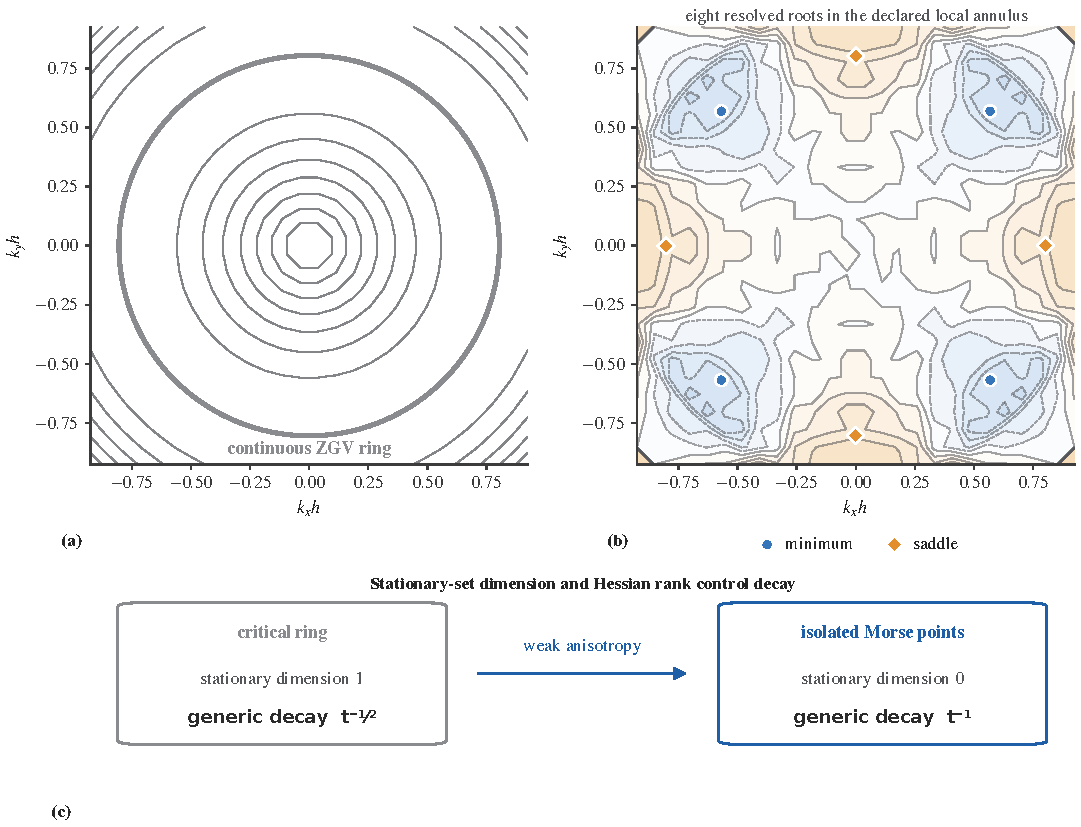
\includegraphics[width=\textwidth]{../figures/main/figure_01_geometry_mechanism.pdf}
  \caption{\FigureOneCaption}
  \label{fig:geometry-mechanism}
\end{figure}

\subsection{Independent spectral verification}

We next test the exact reference with an independent thickness-resolved
calculation, restricted to the same configured local window and tracked
spectral branch.  The generalized Hermitian eigenproblem uses traction-free
natural boundary conditions and no Rayleigh--Lamb determinant.  Thus its
agreement with the exact root checks a distinct numerical representation of
the elastic field.  This is a computation-only verification rather than an
experiment: no measured resonance, fitted material parameter, or laboratory
observable enters the comparison.

The spectral weak form of Eq.~\eqref{eq:spectral-weak-form} resolves all
displacement components through the thickness.  Branch continuity is enforced
by the mass-weighted overlap procedure in Algorithm~\ref{alg:mode-tracking},
and queries are rejected when the local separation condition in
Eq.~\eqref{eq:eigengap-rejection} is not met.  Across the declared order
sweep, the normalized eigen-residual of
Eq.~\eqref{eq:normalized-eigen-residual}, the mass-orthogonality defect of
Eq.~\eqref{eq:mass-orthogonality-defect}, and the exact-reference errors remain
small while the relative eigengap stays
open.  This simultaneously checks branch identity, field resolution, and the
simple-eigenvalue hypothesis used by Theorem~\ref{thm:morse-bott-ring}; it is
not a claim about branches outside the tracked window.  Spectral guided-wave
discretization itself is established methodology \citep{adamou2004spectral}.

Figure~\ref{fig:isotropic-zgv} separates the four pieces of this check.  The
tracked symmetric branch has a local minimum at the computed
$(\ZGVKappa,\ZGVOmega)$ reference; the exact branch and its quadratic form
with curvature $\ZGVCurvature$ agree over the declared local comparison
interval.  The convergence panel reports errors and eigengap
together, preventing apparent frequency agreement from masking branch
coalescence.  Finally, the mass-normalized mode panel shows the
through-thickness component magnitudes and their squared-displacement proxy;
because it plots magnitudes, it is not used as a signed parity test.  These mutually
consistent diagnostics support
the Morse--Bott statement only for the selected uniformly gapped local branch.

\begin{figure}
  \centering
  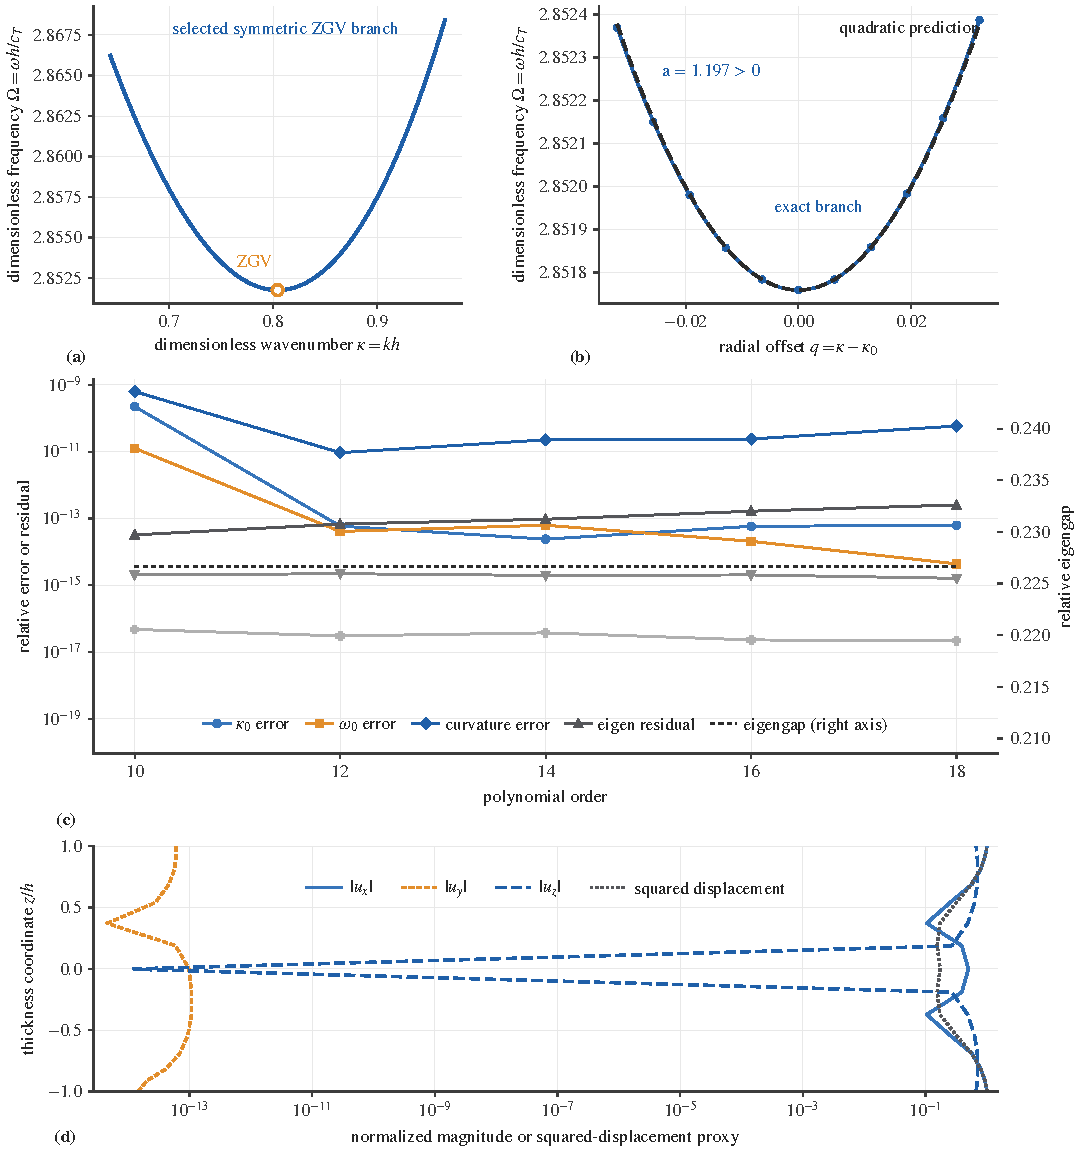
\includegraphics[width=\textwidth]{../figures/main/figure_02_isotropic_zgv.pdf}
  \caption{\FigureTwoCaption}
  \label{fig:isotropic-zgv}
\end{figure}

\section{Symmetry-Breaking Normal Form}

\subsection{Full-elastic angular sensitivities}

% Claim C2
Within the declared one-parameter cubic family, the angular and radial
coefficients were obtained from the full traction-free generalized eigenproblem,
rather than fitted from the eventual critical-point locations.  The general
Hermitian-pencil derivative in Eq.~\eqref{eq:general-frequency-sensitivity}
gave the ring sensitivity \(V(\theta)\), while the complete radial derivative in
Eq.~\eqref{eq:complete-radial-frequency-sensitivity} retained the differentiated
mode, equivalently the reduced-resolvent contribution, in \(B(\theta)\).  This
calculation is restricted to the simple tracked branch and the declared cubic
perturbation; it does not claim a coefficient formula for an arbitrary
anisotropic plate.

The resulting angular potential contained the derived pure fourfold term of
Eq.~\eqref{eq:cubic-vfour}, with signed coefficient
\(V_4=\VFour\).  Here \(V_4\) is the coefficient of the perturbation parameter,
whereas the physical fourfold frequency shift is \(\varepsilon V_4\), as fixed
by Eq.~\eqref{eq:physical-cubic-angular-shift}; the perturbation parameter is
therefore counted once.  Centered full-wave finite differences independently
recovered both \(V(\theta)\) and \(B(\theta)\).  Figure~\ref{fig:angular-sensitivity}
shows the harmonic reconstruction, the coefficient-to-shift convention, and
the finite-difference closure.  These checks make the full-elastic coefficient
closure, rather than symmetry alone, the quantitative input to the unfolding.

\begin{figure}
  \centering
  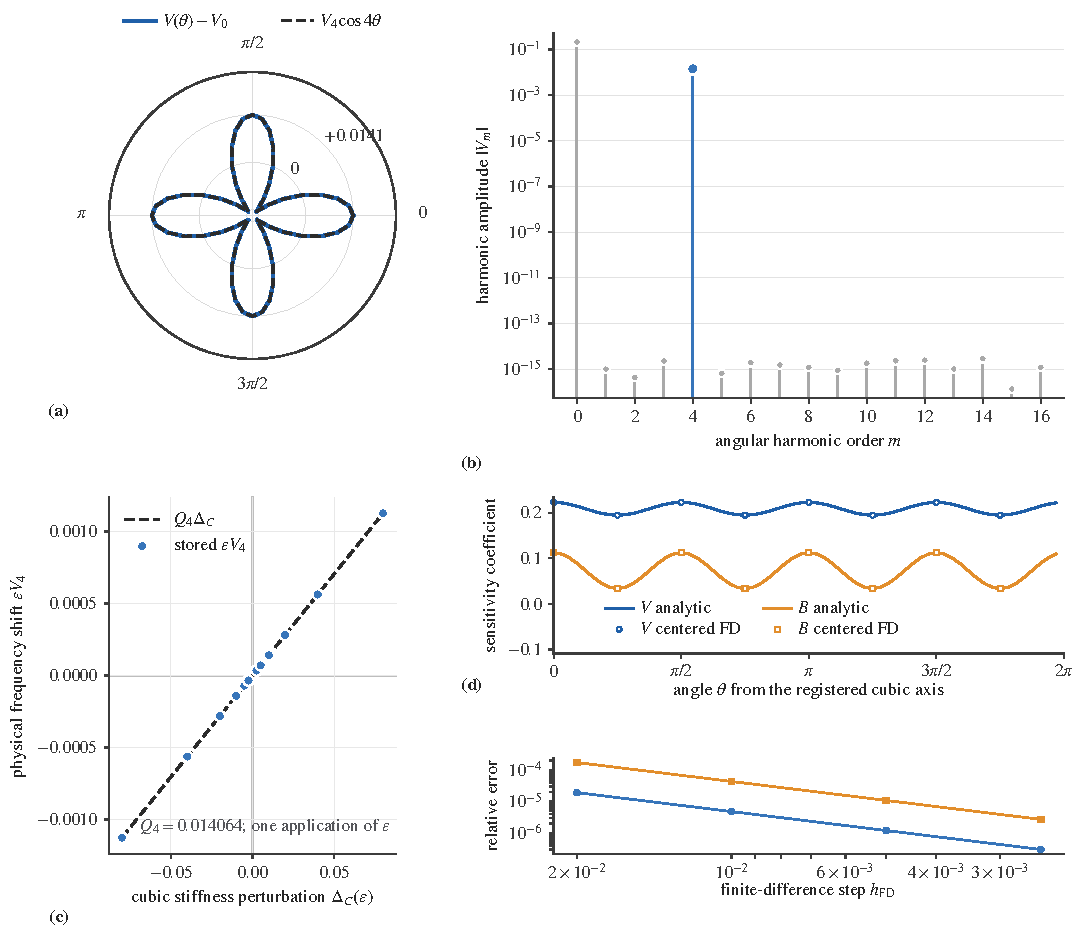
\includegraphics[width=\textwidth]{../figures/main/figure_03_angular_sensitivity.pdf}
  \caption{\FigureThreeCaption}
  \label{fig:angular-sensitivity}
\end{figure}

\subsection{Normal form and splitting theorem}

% Claim C3
Under the controlled weak-anisotropy hypotheses, eliminating the radial
stationarity equation reduced the local dispersion to an angular problem in
the declared local annulus.  Theorem~\ref{thm:anisotropic-normal-form} and
Eq.~\eqref{eq:controlled-anisotropic-normal-form} retain the radial quadratic,
the angular sensitivity, the mixed radial--angular coefficient, and a
derivative-level remainder.  The implicit radial graph in
Eq.~\eqref{eq:radial-shift} is unique in this neighborhood; substituting it
gives the reduced angular frequency of
Eq.~\eqref{eq:reduced-angular-frequency-second-order}.  These steps require a
simple separated eigenvalue and a nonzero radial curvature.

The cubic splitting theorem in Theorem~\ref{thm:cubic-morse-splitting} then
placed the critical angles and radial corrections according to
Eq.~\eqref{eq:cubic-eight-critical-points}.
For every sufficiently small nonzero \(\varepsilon\) with \(V_4\ne0\), the
theorem yields
\MorseMinimumCount{} Cartesian Morse minima and \MorseSaddleCount{} Cartesian
Morse saddles in alternating angular order.  This exact local count depends on
the derived leading harmonic and controlled remainder, not on \(C_{4v}\)
symmetry by itself and not on a global survey of every dispersion branch.

The retained isotropic radial curvature is positive.  Consequently, the sign
of the tangential curvature distinguishes the Cartesian Hessian classes: two
positive eigenvalues give a minimum, whereas one positive and one negative
eigenvalue give a saddle.  This inertia statement follows from the exact
polar-to-Cartesian Hessian in Eq.~\eqref{eq:critical-cartesian-polar-hessian}
and its Schur complement in Eq.~\eqref{eq:hessian-schur-inertia}.  A direction
with negative angular curvature is thus not a maximum.  Reversing the sign of
\(\varepsilon V_4\) exchanges the minimum and saddle angular roles while
preserving their alternating organization.  The
four-minimum/four-saddle pattern is known in anisotropic ZGV calculations
\citep{kiefer2023beating,kiefer2025skewing}; the contribution here is the
full-elastic coefficient closure together with a controlled local explanation
of why that pattern follows for this perturbation family.

\subsection{Eight resolved critical points}

% Claim C4
We restricted the full-wave search to the declared local annulus on the
tracked full-elastic branch.  The thickness discretization retained all three
displacement components.  Within this scope, the search found eight resolved roots,
comprising \MorseMinimumCount{} minima and \MorseSaddleCount{} saddles.  Every
accepted root satisfied the gradient-resolution condition associated with
Eq.~\eqref{eq:critical-point-uncertainty}, and its Cartesian Hessian eigenvalues
remained separated from their numerical discrepancy estimate.  Candidate-grid
refinement preserved the locations and alternating types.  This is a
finite-resolution local realization on one branch, not a proof of exhaustive
continuum enumeration.  In particular, the winding and grid checks cannot
exclude an unresolved opposite-index pair between candidate nodes.  Exact
four-plus-four cardinality is reserved for the sufficiently-small theorem
above, while the computed result is reported as eight refinement-stable roots.

The artifact field \texttt{morse\_index} stores the gradient, or Poincar\'e,
index rather than the number of negative Hessian eigenvalues: each resolved
minimum contributes \(+1\), each saddle contributes \(-1\), and the total is
zero.  The outer-minus-inner gradient winding agreed with this point-index sum
under Eq.~\eqref{eq:annular-index-certificate}, while both annular boundaries
remained noncritical.  Figure~\ref{fig:morse-points} displays the stored refined
coordinates, Hessian inertia, and perturbative location errors.  Point type was
assigned only when the Cartesian Hessian signs exceeded their discrepancy
estimate; it was not inferred from the appearance of interpolated contours.

\begin{figure}
  \centering
  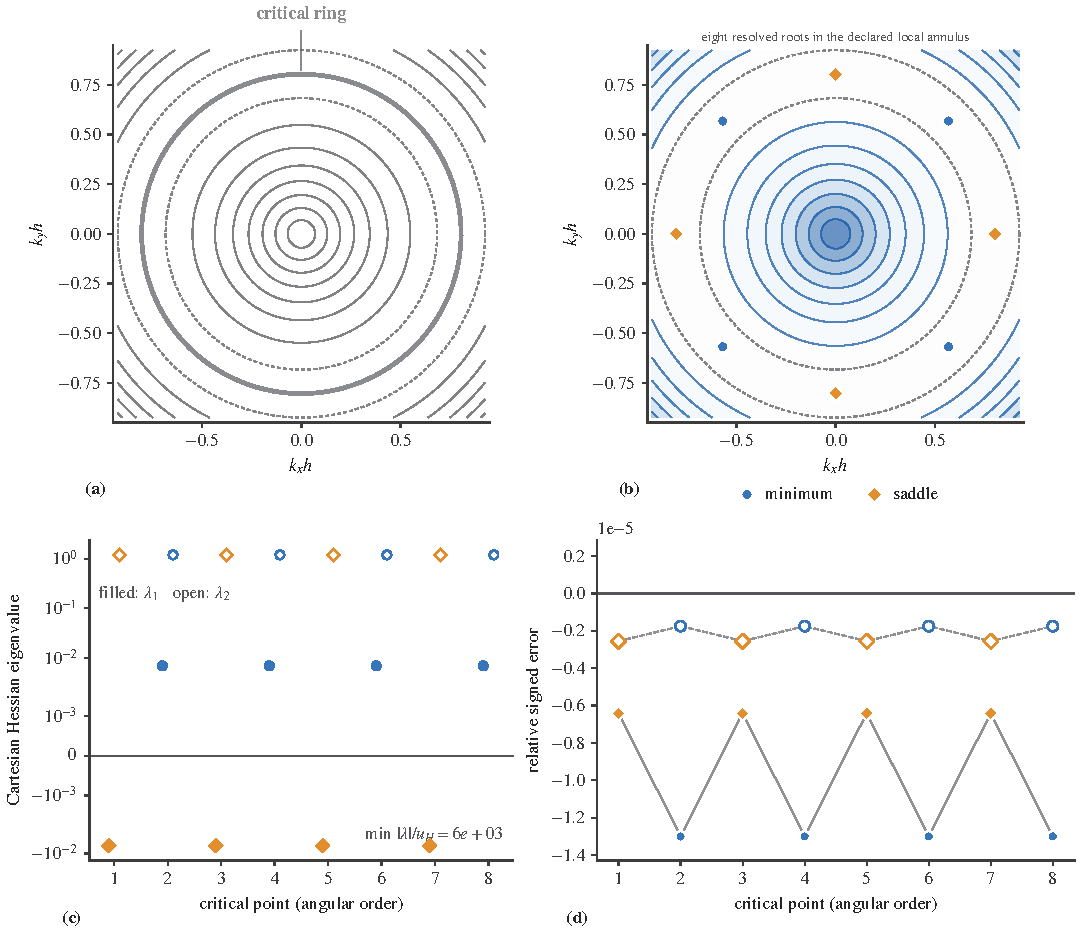
\includegraphics[width=\textwidth]{../figures/main/figure_04_morse_points.pdf}
  \caption{\FigureFourCaption}
  \label{fig:morse-points}
\end{figure}

\subsection{Scaling and sign checks}

% Claim C5
Within the predeclared weak-anisotropy sequence, compensated full-wave data
approached the radial prediction in Eq.~\eqref{eq:radial-shift}, and the
minimum--saddle critical-frequency separation followed
Eq.~\eqref{eq:cubic-minimum-saddle-separation}.  The stored log--log slope of
the separation was \SplittingSlope, consistent with first-order scaling, while
the frequency remainder slope was \RemainderSlope, consistent with a
second-order residual.  These statements are restricted to the resolved
nonzero coefficients and the declared perturbation sequence; they are not
extrapolations to a finite material anisotropy.

The compensated radial shifts and frequency remainders provide the primary
coefficient-level checks because they retain the predicted limits directly.
In particular, division by the signed perturbation approaches the full-elastic
coefficient ratio \(-B(\theta)/a\) on both angular families.
The fitted slopes are secondary summaries of those same predeclared data, not
standalone evidence or a plot-selected scaling window.  Sign reversal supplied
an independent control: changing \(\varepsilon V_4\) exchanged the angular
roles without changing the minimum and saddle counts.  Figure~\ref{fig:perturbation-scaling}
reports the complete sequence, the first- and second-order compensated
quantities, and the role-reversal check.

\begin{figure}
  \centering
  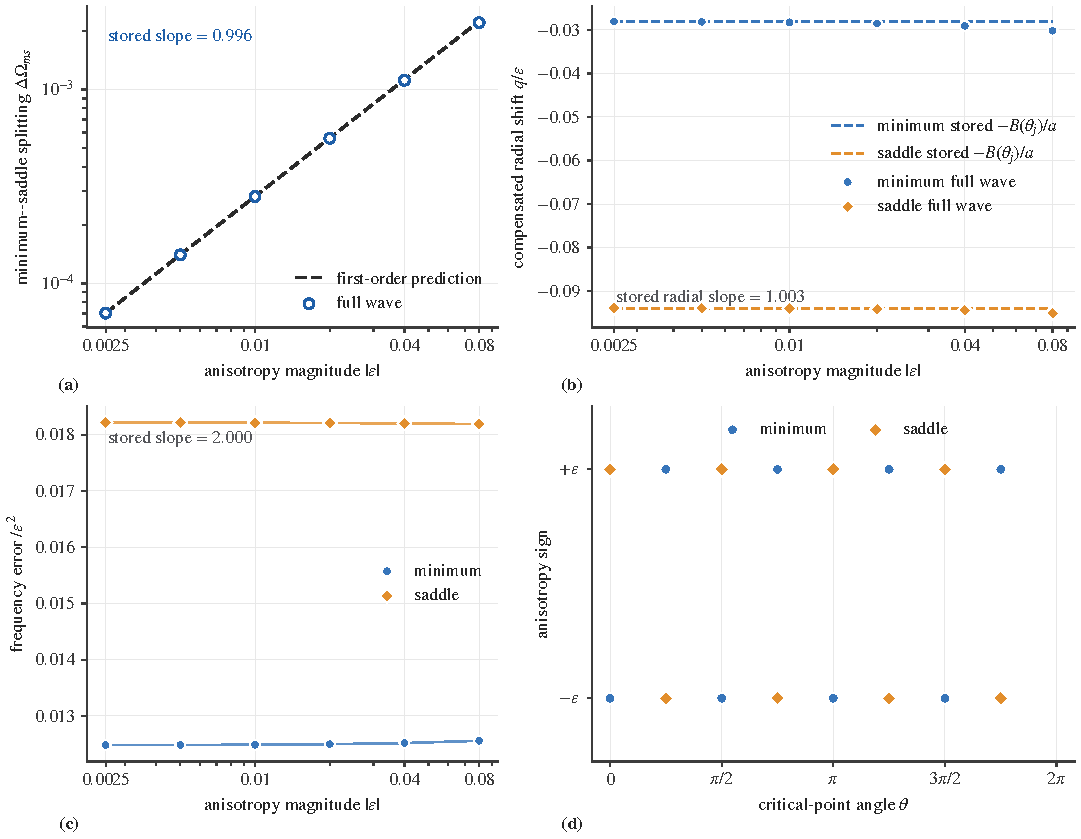
\includegraphics[width=\textwidth]{../figures/main/figure_05_perturbation_scaling.pdf}
  \caption{\FigureFiveCaption}
  \label{fig:perturbation-scaling}
\end{figure}

\section{Coefficient-Resolved Temporal Crossover}

\subsection{Joint-limit Bessel law}

% Claim C6
Within the declared joint-limit window for the nonnodal source and angular
weight class, the undoubled positive-frequency response
\(G^{+}(t;\varepsilon)\) of the tracked branch collapsed onto the
coefficient-resolved Bessel form in
Theorem~\ref{thm:uniform-bessel-crossover}.  Equation~\eqref{eq:uniform-response}
retains the radial \(t^{-1/2}\) factor and angular kernel
\(J_0(\varepsilon V_4t)\), with the full-elastic coefficient
\(V_4=\VFour\).  Here \(t:=t_{\mathrm{phys}}c_T/h\) is dimensionless,
and \(V_4\) is the correspondingly scaled sensitivity coefficient;
\(\varepsilon V_4\) is the finite-\(\varepsilon\) shift in this convention,
and its dimensional value is \((c_T/h)\varepsilon V_4\).  The complex
collapse in Fig.~\ref{fig:decay-crossover} was evaluated
without fitted alignment of amplitude, phase, frequency, or time.
This connects the established isotropic radial decay and anisotropic splitting
without claiming a new Bessel identity
\citep{prada2008power,kiefer2023beating,creagh1996broken,brack1999uniform,
brack2009closed}.

The agreement included the sign-preserving transition coordinate
\(\tau=\varepsilon V_4t\), although the axisymmetric \(J_0\) kernel is even
in that coordinate.  The early declared envelope fit gave the slope
\(\EarlyDecaySlope\), consistent with the radial stationary-phase exponent
before the fourfold angular stationary points were resolved.  Scaled absolute
complex error, rather than relative error, was retained around zeros of the
Bessel factor.  The angular integral producing \(J_0\) is an established
Bessel identity; the result here is its coefficient-resolved realization for
the selected Lamb branch, not a new identity.

\begin{figure}
  \centering
  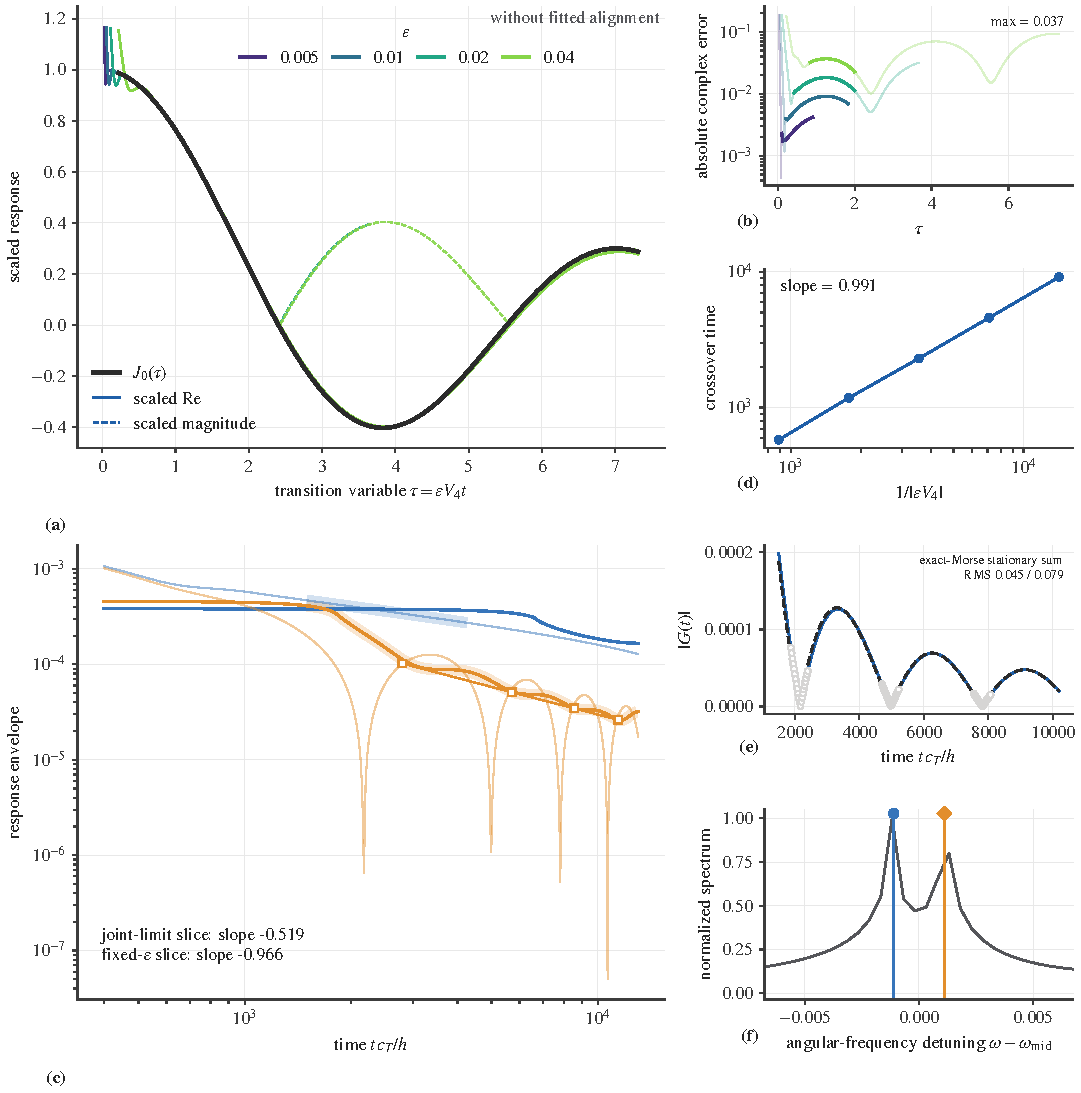
\includegraphics[width=\SixPanelFigureWidth]{../figures/main/figure_06_decay_crossover.pdf}
  \caption{\FigureSixCaption}
  \label{fig:decay-crossover}
\end{figure}

\subsection{Overlap with isolated stationary points}

Under the growing-\(\lvert\tau\rvert\) overlap conditions, but only while the
accumulated second- and higher-order phase corrections remain controlled, the
same branch entered the isolated-point scale
\(O(\lvert\varepsilon V_4\rvert^{-1/2}t^{-1})\).  This conclusion follows from the
independent growing-parameter stationary-phase argument in
Theorem~\ref{thm:growing-bessel-morse-overlap}; the compact-\(\tau\) theorem
cannot be extrapolated to large \(\lvert\tau\rvert\).  The limit and its
explicit error budget are stated in Eqs.~\eqref{eq:growing-overlap-limit}
and \eqref{eq:growing-overlap-error}, while
Eq.~\eqref{eq:bessel-overlap-response} restores the response normalization.
The overlap proof
directly resolves the alternating angular stationary points and recovers the
Cartesian minimum and saddle signature factors within the declared local
annulus.

Expanding the large-argument Bessel factor in this controlled overlap produced
the same coefficient and phases as the corresponding first-order
four-minimum/four-saddle Morse sum in
Eq.~\eqref{eq:bessel-morse-overlap}, not
merely the same decay exponent.  The fourfold multiplicity of each critical
family cancelled the angular-curvature factor, leaving the expected radial and
angular stationary-phase prefactor.  Away from destructive-cancellation times,
a fixed small nonzero \(\varepsilon\) slice has the \(t^{-1}\) time exponent.
Along a joint path, however, the prefactor
\(\lvert\varepsilon V_4\rvert^{-1/2}\) remains explicit and can diverge as the
ring is restored.  Root-mean-square binning is therefore the suitable
cancellation-safe observable.  Figure~\ref{fig:decay-crossover} presents two
numerical asymptotic slices rather than one time trajectory: a
small-perturbation joint-limit slice and a fixed-anisotropy slice.  The plotted
late bins and
\(\LateDecaySlope\) in Fig.~\ref{fig:decay-crossover}, however, belong to the
separate fixed-anisotropy endpoint discussed next; they are not a numerical
joint-path test of the growing-\(\lvert\tau\rvert\) theorem.  The connection
between the slices is the proved growing-\(\lvert\tau\rvert\) overlap above.

\subsection{Fixed-anisotropy Morse endpoint}

% Claim C7
At fixed nonzero anisotropy, and only for resolved nondegenerate critical
points away from the window boundary, standard two-dimensional stationary
phase applied to the exact full-wave Cartesian branch gave the endpoint in
Theorem~\ref{thm:fixed-anisotropy-decay}.  The signed Hessian sum in
Eq.~\eqref{eq:morse-stationary-sum} uses the exact critical frequencies,
modal amplitudes, and Cartesian determinants rather than their first-order
approximations.  It predicts a generic \(t^{-1}\) contribution to the
undoubled positive-frequency response from each nonnodal isolated point; the
physical real response is \(2\operatorname{Re}G^{+}\).  This use of standard
two-dimensional stationary phase follows established guided-wave asymptotics
\citep{velichko2007excitation,chapuis2010focusing,karmazin2013caustics}.

At fixed anisotropy, the full-wave response approached this
parameter-determined sum over the declared comparison window.  Its
root-mean-square envelope gave the slope \(\LateDecaySlope\), as shown in
Fig.~\ref{fig:decay-crossover}.  This endpoint complements the joint-limit
Bessel law: the former keeps \(\varepsilon\) fixed while time increases,
whereas the latter takes a controlled two-parameter limit.  The remainder
\(O_\varepsilon(t^{-2})\) in Eq.~\eqref{eq:morse-stationary-sum} is not uniform
as \(\varepsilon\to0\), so this endpoint does not replace the coalescing-ring
description.

\subsection{Frequency separation and modulation rate}

Within the fourfold family on the tracked branch, the exact minimum and saddle
frequencies appeared as two critical-frequency features of the infinite,
lossless continuum.  Their nonnegative separation in
Eq.~\eqref{eq:critical-frequency-separation} is twice the modulation
angular-frequency magnitude in Eq.~\eqref{eq:signed-modulation-rate}.  This
factor-of-two statement is restricted to the signed two-family modulation and
keeps the feature separation distinct from the magnitude that multiplies the
dimensionless time \(t\)
after the mean carrier has been removed.

At leading order, the separation is \(2\lvert\varepsilon V_4\rvert\), whereas
the modulation magnitude is \(\lvert\varepsilon V_4\rvert\).  The minimum and
saddle signature phases then generate the signed cosine recovered in the
growing-parameter overlap.  The quantitative comparison uses the exact
critical-point frequencies; the spectrum panel of
Fig.~\ref{fig:decay-crossover} is qualitative.  At fixed anisotropy, unequal exact amplitudes and
higher-order phase corrections may deform the cosine into a two-phasor
modulation, but they do not alter the definition of the exact
critical-frequency separation.

\section{Full-Wave Numerical Verification}

\subsection{Convergence and resolution checks}

Within the declared local annulus and on the tracked branch, the isotropic
coordinates and curvature passed the predeclared order-convergence gates.
The eigenpairs and continuation history separately passed the residual,
orthogonality, overlap, and eigengap gates.  The independently computed values
remained consistent with
\(\kappa_0=\ZGVKappa\), \(\Omega_0=\ZGVOmega\), and
\(a=\ZGVCurvature\), while Fig.~\ref{fig:isotropic-zgv} exposes the full
order sequence rather than only its finest member.  This evidence concerns the
selected local branch and does not assert completeness for the dispersion
spectrum outside the configured window.

No coordinate match was accepted alone.  A converged row also had to satisfy
the normalized residual of Eq.~\eqref{eq:normalized-eigen-residual}, the mass
orthogonality defect, the mass-weighted overlap of Eq.~\eqref{eq:mass-mac}, and
the relative separation gate in Eq.~\eqref{eq:eigengap-rejection}.  The
generated Supplementary convergence table reports the final one- and
two-element values beside their declared gates.  Algorithm~\ref{alg:mode-tracking}
supplied the branch history, so apparent coordinate agreement after a branch
switch could not pass this joint check \citep{adamou2004spectral,kiefer2023computing}.

The anisotropic evidence closed a distinct joint gate.  Centered
full-anisotropic differences checked \(V_4=\VFour\) and the differentiated-mode
equation, while Hessian discrepancy estimates and candidate-grid refinement
checked the \(\MorseMinimumCount\)-minimum and
\(\MorseSaddleCount\)-saddle set in
Figs.~\ref{fig:angular-sensitivity} and \ref{fig:morse-points}.  The two
resolution routes are defined in Eqs.~\eqref{eq:differentiated-mode-solve}
and \eqref{eq:critical-point-uncertainty}.  Boundary noncriticality and the
index identity of Eq.~\eqref{eq:annular-index-certificate} then closed the
declared local annulus.  Together these checks support a resolved local set
on one branch, not a global enumeration or laboratory evidence.

\subsection{Response and phase accuracy}

For the declared joint-limit rows and the separate fixed-anisotropy row,
independent full-wave polar-grid refinements converged while the maximum
accumulated inter-resolution phase-discrepancy estimator remained
\(\MaxPhaseError\), below its declared acceptance threshold.  Each production
grid rebuilt and retracked its own spectral surface
before applying the Cartesian-measure quadrature in
Eq.~\eqref{eq:polar-green-quadrature}.  The nested subsampling stored in the
auxiliary convergence artifact is therefore a diagnostic only, not a
substitute for these independent production surfaces.

The accumulated inter-resolution phase-discrepancy estimator in
Eq.~\eqref{eq:phase-error-certificate} combines the local nested-order
frequency difference with the common-node difference between successive polar
grids.  It restricts the accepted reported window by comparing computed
resolutions; without a continuum enclosure, it does not bound the unknown
continuum phase error.  Figure~\ref{fig:decay-crossover} shows that the complex
response and fixed-anisotropy comparison passed this same declared consistency
gate.

The masks fixed before response evaluation in Eq.~\eqref{eq:fit-masks} gave an
early decay slope
\(\EarlyDecaySlope\) and a late decay slope \(\LateDecaySlope\).  The early
fit uses only the smallest perturbation row before angular stationary points
are resolved, whereas the late fit uses complete half-open root-mean-square
modulation bins in the fixed-anisotropy row.  The fitted log--log intercept is
a nuisance parameter for exponent estimation; it is not an adjustment of the
transition or exact-Morse response curves, which use no fitted alignment.

\subsection{Source and window robustness}

The declared robustness sweep varied the Gaussian source radius only within
its declared range.  A separate sweep varied the width of the local window in
wavenumber.  The response norm changed by a bounded amount, while the baseline
normalization and localization at the widest window boundary were preserved.
Every declared pair was evaluated from the stored branch surface.  This check
concerns source and truncation sensitivity, rather than a new decay exponent or
critical-point completeness.  The full sweep and its boundary-weight
diagnostic are reported in the Supplementary Information.

The baseline row is included in both one-parameter sweeps, so every reported
difference has a common normalization.  The window check also bounds the
weighted contribution at the radial endpoints, limiting the possibility that
the response trend is created by abrupt branch truncation.  These controls
support the interpretation of Fig.~\ref{fig:decay-crossover} without replacing
the asymptotic hypotheses or the independent phase-discrepancy check.

\subsection{Silicon stress test}

A separate calculation for a \([0\,0\,1]\)-cut silicon plate recovered an
alternating local minimum--saddle set with resolved Cartesian Hessians and noncritical
annular boundaries, serving only as a finite-anisotropy stress test.  The
calculation repeats the tracked-branch search and the winding procedure of
Eq.~\eqref{eq:annular-index-certificate}, but physical silicon lies outside the
controlled weak-anisotropy sequence used for the coefficient and remainder
claims \citep{prada2009anisotropy,kiefer2023beating}.

Accordingly, this result is reported as numerical robustness of the search,
classification, and boundary-check machinery under a materially larger
constitutive contrast.  It supplies neither evidence for the weak-parameter
scaling laws nor a count over the complete silicon dispersion surface.  The
local alternating organization is consistent with earlier anisotropic ZGV
computations, while the claims of this study remain attached to the declared
perturbative family and its explicitly tracked branch.
The corresponding contours, refined points, Hessian inertia, and boundary
margin are reported in the Supplementary Information.

\section{Discussion}

\subsection{Geometry and noncommuting limits}

Within the controlled weak-cubic family and the declared local annulus, the
essential change is geometric rather than a uniform frequency displacement.
The local Morse--Bott ring unfolds into isolated Morse minima and saddles.
The isotropic ZGV critical ring is Morse--Bott: radial localization is
nondegenerate, but continuous rotation leaves a tangential Hessian zero mode
(Theorem~\ref{thm:morse-bott-ring}).  Cubic anisotropy lifts that zero mode and
organizes the local stationary set into alternating Cartesian Morse points
(Theorem~\ref{thm:cubic-morse-splitting}).  The extra nondegenerate direction
adds angular stationary phase to the existing radial stationary phase.  This
explains why the ring and point regimes carry different time exponents without
describing the change as a phase transition.

The two exponents belong to noncommuting limits.  Write
\(\alpha=\varepsilon V_4\).  The ring-scale response is proportional to
\(t^{-1/2}J_0(\alpha t)\), whereas the isolated-point scale in the controlled
overlap is \(\lvert\alpha\rvert^{-1/2}t^{-1}\).  The latter prefactor follows
from the tangential Hessian curvature in
Eq.~\eqref{eq:overlap-hessian-signatures}; point multiplicity cancels the
fourfold curvature factor but not \(\lvert\alpha\rvert^{-1/2}\).  Its growth as
\(\alpha\to0\) signals loss of uniformity when the points coalesce back into a
ring, not divergence of the physical solution.  At
\(t\sim\lvert\alpha\rvert^{-1}\), both asymptotic scales are of order
\(\lvert\alpha\rvert^{1/2}\), as summarized in
Eq.~\eqref{eq:noncommuting-green-limits}.

The joint-limit Bessel law and fixed-anisotropy exact-Morse sum are therefore
complementary.  The
uniform Bessel theorem controls compact \(\tau=\alpha t\)
(Theorem~\ref{thm:uniform-bessel-crossover}); its large-parameter edge is
matched only through the separately proved growing-\(\lvert\tau\rvert\)
overlap and Eq.~\eqref{eq:bessel-overlap-response}.  At fixed nonzero
anisotropy, the exact-Morse theorem instead uses full critical frequencies,
amplitudes, and Cartesian Hessians (Theorem~\ref{thm:fixed-anisotropy-decay}).
Its remainder is not uniform as \(\varepsilon\to0\), while a first-order
Bessel phase is not indefinitely accurate at fixed \(\varepsilon\).  Neither
formula can be substituted for the other outside the regime it controls.

\subsection{Relation to prior work}

Within the scope of this comparison, both endpoint geometries are established
results rather than discoveries of the present study.  The isotropic ZGV
critical ring and its \(t^{-1/2}\) response follow the classical Lamb-wave
setting \citep{lamb1917waves,prada2008local,prada2008power}.  Directional
anisotropic shifts were also established \citep{prada2009anisotropy}, and
isolated anisotropic ZGV points were previously reported.  In particular, the
four minima and four saddles were previously reported together with their
interference, and beating responses were already reported for cubic silicon
\citep{kiefer2023beating,kiefer2025skewing}.  Full-spectrum algorithms for
locating such points are likewise prior infrastructure
\citep{kiefer2023computing}.

The distinction of the present calculation is the controlled,
coefficient-resolved link between those known endpoints.  Morse--Bott
classification and perturbation are established mathematics
\citep{bott1954critical,banyaga2013cascades}.  Here transverse nondegeneracy is
verified on the exact Lamb determinant and independently on the tracked
elastic branch.  The fourfold coefficient is obtained from the full
generalized-eigenvalue sensitivity, and the radial coefficient retains the
differentiated-mode contribution.  Finite differences, compensated radial
shifts, remainder scaling, sign reversal, Cartesian Hessian inertia, and
annular index closure then test the reduction.  Thus the local four-plus-four
result follows from computed coefficients and controlled remainders, not from
point-group symmetry alone or from fitting the final critical locations.

The asymptotic tools also have clear precedents.  Broken-symmetry uniform
approximations with Bessel modulation connect continuous families and isolated
objects in other wave settings \citep{creagh1996broken,brack1999uniform,
brack2009closed}.  Two-dimensional stationary phase is standard and has been
used for anisotropic guided-wave radiation
\citep{velichko2007excitation,chapuis2010focusing,karmazin2013caustics}.
Accordingly, the contribution is neither a new Bessel identity nor a new
stationary-phase theorem.  It is their fully normalized Lamb-wave realization
with an elasticity-derived Bessel argument, an explicit phase-validity window,
and a constant-and-phase match to the first-order Morse overlap.  Separately,
the fixed-anisotropy endpoint is compared numerically with the exact-Hessian
point sum without fitted amplitude, phase, frequency, or time shifts.

\subsection{Scope and boundary statements}

The canonical Bessel law holds only within the specified nonnodal source and
angular-weight class.  A general source and its angular weight jointly produce
the Fourier--Bessel series of Eq.~\eqref{eq:weighted-bessel-series}; the leading
kernel need not reduce to a single \(J_0\) term.  If the ring amplitude
vanishes, or if a detector is nodal at a particular Morse point, the leading
contribution changes as described in Supplementary
Section~\ref{rem:nodal-channels}.
Cancellation times do not alter the generic exponent, but they do make a
pointwise relative error or local slope ill conditioned.  The declared
source-radius and window sweeps support robustness only over their declared
ranges, not source independence.

The generality of the result has two levels.  At theorem level, any simple,
uniformly gapped finite-radius branch with nonzero radial curvature and a
dominant nonzero fourfold perturbation coefficient has the same local
Morse--Bott-to-Morse structure and exact sufficiently-small four-plus-four
count under the stated remainder hypotheses.  A pure leading fourfold phase,
together with the declared nonnodal source and phase-remainder conditions, is
additionally required for the single-\(J_0\) law and its matched asymptotic
regimes; generic higher harmonics change the angular canonical integral.  At
instance level, coefficient values,
finite-resolution roots, and response comparisons are demonstrated for one
selected Lamb branch and one cubic perturbation family.  The silicon stress
test assesses only the search and classification workflow.

The geometric count is also restricted to one simple branch in the declared
local annulus.  Branch contamination is controlled here by tracking and the
eigengap gate of Eq.~\eqref{eq:eigengap-rejection}; if the eigengap closes, a
scalar sensitivity and reduced resolvent no longer suffice.  Degenerate,
matrix-valued perturbation theory would then be required.  Likewise, zero
radial curvature, a zero-wavenumber stationary point, or a singular exact
Hessian would demand a different canonical scaling.  The computed local count
does not enumerate every Lamb or shear-horizontal branch.

Fourfold symmetry alone does not fix the number of points.  The pure leading
fourfold term is a result of the declared first-order cubic family.  If the
coefficient \(V_4\) is zero, higher harmonics or the second-order effective
angular potential can control the splitting; competing higher harmonics can
also change the root count.  The coefficient \(B\) is not part of the
controlled remainder: the explicit \(\varepsilon qB\) term controls the radial
shift, and \(B\) enters the phase-error and overlap budget through the effective
second-order phase.  Omitting \(B\) therefore changes both the critical
locations and temporal validity.  These cases require a new
coefficient audit rather than extrapolation of the present four-plus-four
formula.

Neither temporal approximation is indefinitely phase accurate outside its
declared late-time window.  Compact-\(\tau\) collapse, the growing-parameter
overlap, and the fixed-anisotropy comparison impose different error
conditions.  The accumulated inter-resolution phase-discrepancy estimator in
Eq.~\eqref{eq:phase-error-certificate} restricts the accepted numerical time
window but does not bound the unknown continuum phase error.  The operational
crossover time in Fig.~\ref{fig:decay-crossover} is found inside a
theory-centred bracket and is therefore a consistency diagnostic, not
independent evidence for inverse-rate scaling; the complex Bessel collapse is
the primary numerical test.  Critical-frequency features in
the lossless continuum should not be interpreted as discrete resonances, and
their exact separation remains twice the defined modulation magnitude.

Finally, the present model is a linear, infinite, homogeneous, lossless plate.
Damping generally introduces complex dispersion and additional decay; finite
boundaries introduce reflections and a discrete modal spectrum; layers,
interfaces, and defects add branches, scattering, and new angular weights.
Each extension requires renewed branch
projection, coefficients, and phase-error analysis.  The finite-anisotropy
silicon stress test is only a robustness check on search, classification, and
boundary consistency checking.  It supplies no weak-parameter theorem and no
global point count.  This computation-only study includes no experiments.

\subsection{Nonlinear amplitude equations are a separate problem}

The normal form used here is only a linear spectral reduction, not a nonlinear
amplitude equation.  Its frequency sensitivities and dispersive exponents
describe propagation after an impulsive load under the linear constitutive
model.  They do not contain nonlinear coupling, saturation, drive-dependent
detuning, mode competition, or pattern selection.  In particular, the local
Morse geometry can organize the linear spectral input to a later theory, but
it does not determine nonlinear states or their stability.

Nonlinear amplitude equations are therefore a separate problem.  Such a study
would require a nonlinear constitutive law, nonlinear traction conditions, a
multiscale solvability calculation, and declared scalings for forcing,
damping, and detuning.  Resonant projections and coupling coefficients would
have to be derived independently, followed by stability analysis.  None of
those equations or coefficients is obtained from the present Green response,
and no nonlinear saturation or pattern-selection result is inferred here.

\section{Methods}

\subsection{Governing equations and nondimensionalization}

We considered an infinite homogeneous elastic plate occupying
\(\mathbb R^2\times[-h,h]\), with density \(\rho\), elasticity tensor
\(C_{ijkl}\), and traction-free faces.  For a plane-wave component
\(\boldsymbol u=\boldsymbol U(z)\exp[\mathrm i(k_xx+k_yy)-\mathrm
i\omega t]\), the strong problem is
\(\partial_j(C_{ijkl}\partial_lu_k)=\rho\,\partial_t^2u_i\), with
\(\boldsymbol\sigma\boldsymbol n=0\) at \(z=\pm h\).  The reference
isotropic solid has \(\lambda=2\), \(\mu=1\), \(\rho=1\), and \(h=1\).
The shear speed is \(c_T=\sqrt{\mu/\rho}\); reported wavenumber, frequency,
and time are \(\kappa=h k^{\rm phys}\),
\(\Omega=h\omega^{\rm phys}/c_T\), and \(t=c_Tt^{\rm phys}/h\).
Consequently, every plotted coordinate and fitted time is dimensionless.
The signed parameter \(\varepsilon\) multiplies the declared cubic
constitutive perturbation at fixed density; it is not a frequency shift.

The isotropic symmetric branch was first computed from the desingularized
Rayleigh--Lamb determinant, rather than from a plate approximation.  Its first
\(S_1\)-ZGV root in the declared search window was obtained at 80-decimal
working precision from the
simultaneous determinant and radial-derivative equations.  Implicit
differentiation supplied the radial curvature.  The selected root and
curvature then served as independent regression targets for the
thickness-resolved solver.  The full determinant construction,
desingularization at the shear cutoff, and Morse--Bott Hessian calculation are
given in Supplementary Section~\ref{sec:isotropic-rayleigh-lamb-derivation}.

\subsection{Spectral solvers}

The three displacement components were discretized only through the
thickness by a Legendre--Gauss--Lobatto (GLL) spectral element method.  The
weak form retains the face traction as its natural boundary term; no face
degree of freedom is constrained and no penalty is added.  Stiffness and mass
were assembled by collocated GLL quadrature in the Mandel strain convention.
The production homogeneous-plate mesh uses one element on \([-h,h]\); a
two-element mesh split at \(z=0\) is an independent assembly check.  The
generalized Hermitian problem
\(\boldsymbol K\boldsymbol u=\omega^2\boldsymbol M\boldsymbol u\) was solved
for the lowest 12 modes with SciPy's generalized-Hermitian \texttt{gvx}
driver.  Eigenvectors were mass normalized.  Matrix Hermiticity, mass
orthogonality, and the normalized eigen residual were tested at every declared
convergence order.

All first and second derivatives of \(\boldsymbol K\) with respect to
\((k_x,k_y)\) were assembled analytically from the wavevector-affine strain
matrix.  Absolute frequency and gradient discrepancy estimators were the
differences between answers at orders \(p\) and \(p+4\).  These inter-order
quantities are empirical resolution indicators, not bounds on the unknown
continuum errors.  The relative estimator used by the eigengap gate was the
maximum of that nested-order eigenvalue discrepancy and the two eigen
residuals.  The committed full profile uses order
pairs 12/16 for the isotropic artifact, 10/14 for the critical-point, scaling,
and Green artifacts, and 12/16 for the silicon stress test; convergence sweeps
the pairs 6/10 through 14/18.  The sensitivity artifact uses order 10 and is
checked by independent physical finite differences rather than a 10/14 pair.  The exact
weak form, derivative matrices, residual definitions, and all fixed gates are
specified in Supplementary Section~\ref{sec:spectral-numerics}.

\subsection{Mode tracking and sensitivities}

Parity identifies the symmetric branch in the independent isotropic validation.
Production angular anchors were seeded by proximity to the exact target
frequency and then continued by a mass-weighted modal assurance criterion.  Near a close pair,
tracking used the complete connected eigenvalue cluster and its principal
subspace overlap before phase alignment.  Eight endpoint-free angular anchors
were constructed independently at orders \(p\) and \(p+4\); closure of the
angular loop required both scalar MAC and the least principal cosine to be at
least \(1-10^{-8}\).  Inward and outward radial rays were continued separately
from each ring anchor.  Samples were rejected when the selected cluster
touched the top of the 12-mode solve or when the relative eigengap was no more
than ten times the relative eigenvalue discrepancy estimator.  This eigengap
gate is a method hypothesis: no scalar sensitivity or Hessian was accepted
through a numerically unresolved crossing.

The generalized-eigenvalue sensitivity was evaluated at fixed mass norm by
the Hellmann--Feynman contraction.  The angular function \(V(\theta)\) and its
mean and fourth harmonic, \(V_0\) and \(V_4\), were computed on 64
endpoint-free angles.  The mixed radial coefficient \(B\) retained the
differentiated-mode contribution.  The mode derivative was obtained from a
bordered reduced-resolvent system with the mass-gauge constraint, and both the
equation and gauge residuals were required to be below \(10^{-8}\).  A centered
full-wave difference in \(\varepsilon\) checked \(V(\theta)\), and a mixed
\((\varepsilon,q)\) difference checked \(B(\theta)\), both with
\(\Delta\varepsilon=\Delta q=0.0025\).  An independent tensor-product step sweep
\(0.02,0.01,0.005,0.0025\) checked convergence.  Supplementary
Section~\ref{sec:anisotropic-morse-derivation} gives the complete
generalized-pencil algebra, rotated cubic contraction, normal form, and Morse
splitting proof.

\subsection{Critical-point search and annular consistency check}

Critical points were searched only on the tracked branch inside the annulus
\((1-f_A)k_0\leq|\boldsymbol k|\leq(1+f_A)k_0\), with \(f_A=0.15\).
Every polar cell in which both radial and tangential gradient components
bracketed zero supplied a seed.  Each seed was refined in Cartesian
coordinates by \texttt{scipy.optimize.root} with the default Powell hybrid
method, a Richardson Cartesian Hessian from steps \(h_H\) and \(h_H/2\) as
Jacobian, and solver tolerance
\(10^{-11}\).  A root outside the annulus or with a gradient residual exceeding
its nested-order gradient-discrepancy estimator was rejected.  Roots were
merged only within the propagated, capped position-resolution radius.

The full calculation repeated the candidate search on \(5\times16\) and
\(9\times32\) radial-by-angular grids.  The Hessian was Richardson extrapolated
from centered gradient differences with full-profile step \(10^{-3}\); a
classification was accepted only if its least absolute eigenvalue exceeded
ten times the Hessian discrepancy estimate.  Counts, kinds, locations,
frequencies, and Hessian eigenvalues had to agree under candidate-grid
doubling.  An
independent annular check sampled each boundary at 32 and 64 angles, required a
gradient norm separated from its discrepancy estimate, stable boundary
winding, angular increments below \(\pi/2\), and equality between outer-minus-inner
winding and the sum of point indices.  The \(\varepsilon<0\) search was repeated
on an angularly offset candidate grid.  This is a finite-resolution
local-annulus consistency check, not an exhaustive continuum enumeration and
not a global enumeration of every Lamb and shear-horizontal branch.  Index
closure alone also cannot exclude an unresolved pair of
opposite-index critical points between candidate-grid nodes; candidate-grid
doubling, symmetry-offset repetition, and Hessian separation supply the
additional controls used here.

A separate finite-anisotropy stress test used crystal axes
\(x\parallel[100]\), \(y\parallel[010]\), and \(z\parallel[001]\), so the
plate normal was [001].  The constants \(C_{11}=165.7\), \(C_{12}=63.9\), and
\(C_{44}=79.6\) GPa followed the published single-crystal elasticity record
\citep{zhang2014silicon}.  The calculation normalized stiffness by \(C_{44}\),
set \(\rho=h=1\), and reported frequency in
\(\sqrt{C_{44}/\rho}/h\).  It exercised the search and annular consistency check
under stronger constitutive contrast and was not used to validate the
weak-\(\varepsilon\) theorem.

\subsection{Green-function quadrature and fit masks}

The positive-frequency response was projected onto the tracked branch for a
normal impulsive source and top-face normal detector.  The modal amplitude
was \(\mathrm i|u_z(h)|^2/(2\omega)\).  A Gaussian source factor with
\(R/h=0.5\) and a fixed branch window
\(\exp[-(q/\sigma)^8]b_\sigma(q)\), where \(q=|\boldsymbol k|-k_0\) and
\(\sigma/k_0=0.15\), were applied.  The deterministic \(C^\infty\) taper
\(b_\sigma\) equals one for \(|q|\leq1.25\sigma\), uses the standard flat
\(\exp(-1/x)\) transition, and is exactly zero for
\(|q|\geq1.5\sigma\).  Thus the integration interval
\([-1.5\sigma,1.5\sigma]\) contains the complete compact support and has no
endpoint contribution.  Direct integration used the Cartesian
Fourier measure with radial polar Jacobian \(k_0+q\), an endpoint-free
trapezoidal rule in angle, and composite
Simpson quadrature in radius.  No Bessel function entered this full-wave
quadrature.  The full profile rebuilt independent tracked surfaces on
\(129\times32\), \(257\times64\), and \(513\times128\) grids for the uniform
comparisons at \(\varepsilon\leq0.04\); the fixed \(\varepsilon=0.08\)
comparison used twice as many angular nodes.
For every response row, the stationary-point search used an annular half-width
\(1.55\sigma=0.2325k_0\), strictly larger than the direct support
\(1.5\sigma=0.225k_0\), on a \(15\times32\) candidate grid.  Boundary/index
checks used 16 and 32 angular nodes.  Every resolved stationary point in this
larger domain was evaluated with the same compact taper and included in the
fixed-Morse sum; the domain, margin, point counts, and contribution counts are
stored in the Green sidecar.
The computed time axis was \(t_n=400+25n\), \(0\leq n\leq504\), for
\(\varepsilon\in\{0.005,0.01,0.02,0.04,0.08\}\).

Fit masks were fixed in code before response evaluation.  The early slope
used \(\varepsilon=0.005\), \(t\geq1500\), and
\(0.10\leq|\varepsilon V_4t|\leq0.30\).  The fixed-anisotropy late slope used
complete half-open minimum--saddle modulation periods beginning at \(t=1500\),
with at least three samples per period and four periods.  Ordinary least
squares was applied to \(\log t\) and the logarithm of the predeclared RMS or
demodulated amplitude.  The fitted intercepts were diagnostic only: the Bessel and
exact-Morse comparisons used no fitted alignment of amplitude, phase, carrier
frequency, or time.  The full response was accepted only if the three-grid
complex error contracted and the accumulated inter-resolution
phase-discrepancy estimator satisfied the declared
\(t_{\max}\max|\delta\omega|\leq0.05\) rad acceptance test.  This estimator
compares computed resolutions and does not bound the unknown continuum phase
error.  Supplementary
Section~\ref{sec:green-function-asymptotics} derives the normalized response
and all asymptotic regimes; Supplementary Section~\ref{sec:spectral-numerics}
specifies the quadrature, fit masks, cancellation exclusion, and error gates.

\subsection{Reproducibility}

Reference physical parameters and cross-stage acceptance limits are versioned
in \path{config/reference.yaml}; stage-specific grids, masks, and thresholds
are versioned in the workflow source and repeated in artifact sidecars.  The
interpreter is pinned by \path{.python-version}, and dependency resolution is
fixed by \path{uv.lock}.  The seven workflow stages write paired NPZ arrays and
JSON sidecars containing array schemas, units, commands, input hashes, source
and lock hashes, tolerances, measured diagnostics, and SHA-256 output hashes.
Figures read only qualified artifacts, export their plotted source CSV files,
and pass a strict geometry, provenance, and typography audit.

The committed environment used uv 0.11.19, Python 3.12.13, NumPy 2.5.1, SciPy
1.18.0, SymPy 1.14.0, Matplotlib 3.11.0, mpmath 1.3.0, and PyYAML 6.0.3.
Supported Python versions and dependency ranges remain declared in
\path{pyproject.toml}; the interpreter pin and lock file, not those ranges,
define the verified Python environment.  PDF compilation used latexmk 4.88,
pdfTeX 1.40.29, and BibTeX 0.99e from TeX Live 2026; these are external build
prerequisites rather than Python dependencies.

From the package root, the currently executable scientific rebuild is

\begin{verbatim}
uv sync --python 3.12.13 --frozen --all-extras
uv run python scripts/reproduce_all.py \
  --profile full --skip-paper
uv run python scripts/export_manuscript_values.py
\end{verbatim}

The full-profile command first runs the complete test suite, then the
isotropic, sensitivity, critical-point, scaling, Green, convergence, and
silicon stages in isolated processes.  It validates each artifact immediately,
validates the provenance manifest, rebuilds the six main and six supplementary
figures and two generated tables, and performs strict figure QA.  The next
command exports the evidence-checked manuscript macros.  The locked compiler
then checks the recorded latexmk, pdfTeX, and BibTeX versions, builds the
Supplement from \path{supplement.tex} before the main text from
\path{main.tex} in two
independently cleaned cycles, applies the strict final-log gate, rejects
nondeterministic PDF metadata, and requires the two cycles to agree byte for
byte:

\begin{verbatim}
uv run python scripts/compile_paper.py
\end{verbatim}

The supplement must be compiled first because the main document imports its
label file.  The smoke profile is a runtime check only; it is not the source of
committed numerical evidence.  Availability boundaries are stated below.

\section{Conclusion}

We connect a known isotropic ZGV critical ring to its known anisotropic
isolated-point endpoint through a coefficient-resolved geometric and temporal
reduction.  Full-elastic sensitivities determine \(V_4\) and \(B\), while the
exact determinant, independent spectral discretization, and centered
finite-difference checks close the coefficient evidence.  The controlled
normal form gives the exact critical-point cardinality for sufficiently small
perturbations, while the finite-resolution calculation resolves the corresponding alternating
minima and saddles with the predicted splitting, radial shift, remainder, and
sign reversal.  Response quadrature that passes the inter-resolution
phase-discrepancy test then connects the Bessel transition to the exact-Hessian
fixed-anisotropy Morse endpoint.  This
connection explains how the change in stationary-set dimension and Hessian rank
adds angular stationary phase and changes the computed temporal power law.  The
response comparison is performed without fitted alignment of amplitude, phase,
frequency, or time.

The two temporal descriptions express noncommuting limits.  In the joint
limit \(\varepsilon\to0\), \(t\to\infty\), with
\(\tau=\varepsilon V_4t=O(1)\), the radially localized ring retains its
\(t^{-1/2}\) factor and acquires the \(J_0(\tau)\) modulation.  At fixed,
resolved nonzero anisotropy, the isolated Cartesian Morse points instead give
the ultimate \(t^{-1}\) signed-Hessian sum, whose remainder is not uniform as
the ring is restored.  The exact minimum--saddle critical-frequency separation
is twice the modulation angular-frequency magnitude; keeping those quantities
distinct prevents a frequency-feature separation from being confused with the
rate that multiplies time.

The validity scope is restricted to one simple tracked branch of a lossless
infinite plate, a declared local annulus, a nonnodal source and weight class,
and the controlled weak-anisotropy family.  The results are computation-only
and make no global count across all branches; the finite-anisotropy silicon
stress test lies outside the asymptotic evidence.
Weak loss, finite boundaries, layered or defective plates, and near-closing
eigengaps require extensions of the coefficient and error analysis.
Nonlinear amplitude equations are a separate problem and belong to a distinct
study rather than to the linear response developed here.

\section*{Data Availability}

All data supporting the conclusions are present in the accompanying source
tree.  Seven qualified artifact pairs---NPZ arrays plus JSON sidecars---and
the auxiliary isotropic validation and convergence records reside in
\path{data/generated}.  A separate source-data directory contains the
machine-readable source data in CSV format plotted in every main and
supplementary figure.  Generated manuscript
tables and \path{data/provenance_manifest.json} are also included.  Artifact
sidecars and the provenance manifest record SHA-256 hashes for qualified inputs
and outputs.  At this pre-deposition stage, no external accession, repository
DOI, or release-wide checksum manifest is available.

\section*{Code Availability}

The accompanying source tree contains all Python source, tests, the reference
configuration, the interpreter pin, the exact dependency lock, figure scripts,
and LaTeX sources required to regenerate the numerical artifacts, figures,
tables, and PDFs.  The current full scientific route is
\texttt{uv run python scripts/reproduce\_all.py --profile full --skip-paper};
the evidence macros and two PDFs are then rebuilt by the explicit commands in
Methods, with the supplement compiled before the main paper.  No proprietary
solver or experimental data are required.


\bibliographystyle{apsrev4-2}
\bibliography{references}

\end{document}
